\chapter{Implementierung}
\label{cha:Implementierung}

\section{Interessante Code-Segmente}

Abbildung~\ref{fig:controller-state-machine} zeigt die Implementierung der State Machine in Python. Hierbei beschreiben die transitions die Zustandsänderungen. Ist beispielsweise der der aktuelle Modus automatisch, so bleibt bei einer Helligkeitsänderung der Modus weiterhin automatisch. Weiterhin wird die Helligkeit aktualisiert und die neue Position der Jalousie eingestellt.
In der for schleife \textbf{for room in blinds} wird eine entsprechende State Machine für jeden Raum erstellt.
\begin{figure}[hbt]
	\centering
	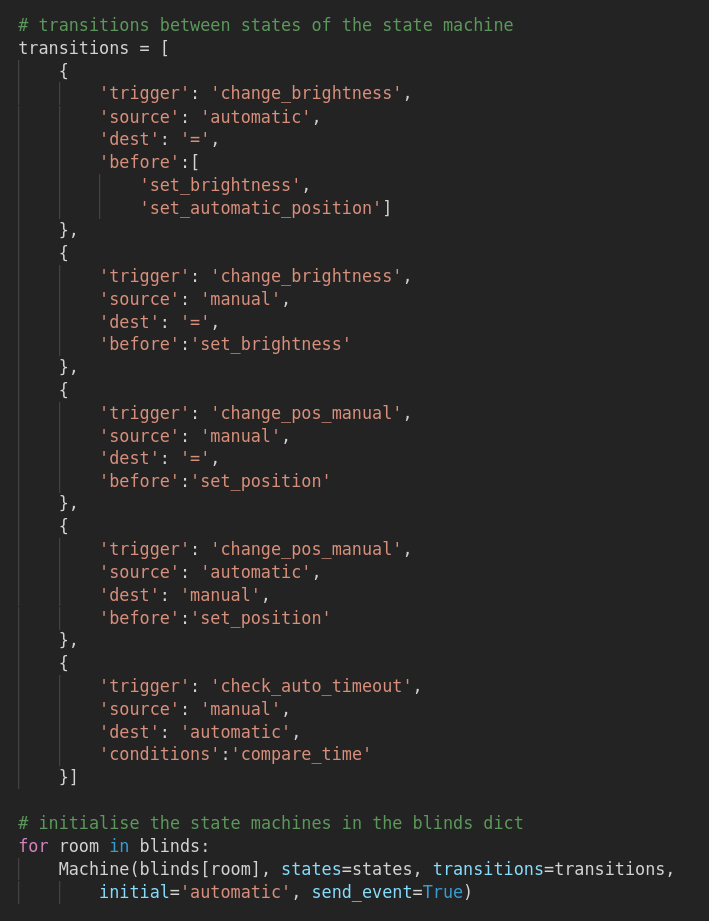
\includegraphics[width=0.5\linewidth]{images/controller-state-machine}
	\caption[Code Segment Controller State Machine]{Controller State Machine}
	\label{fig:controller-state-machine}
\end{figure}

Abbildung~\ref{fig:task} zeigt die Erstellung des Motor Control Task. Motor\_control\_handle wird hier genutzt um den Task im Falle eines Interrupts durch die Endstopps zu stoppen.
\begin{figure}[hbt]
	\centering
	\includegraphics[width=0.5\linewidth]{images/task}
	\caption[Code Segment Task]{Task}
	\label{fig:task}
\end{figure}

Abbildung~\ref{fig:task-calls} zeigt den Aufbau der Hauptfunktion des Sensor Modules. Es werden hier zuerst die Grenzwerte gesetzt bei deren Überschreitung der Hauptprozessor wieder gestartet werden soll. Im Folgenden werden NVS Flash, WiFi und MQTTS initialisiert und das letzte Messergebnis (ulp\_last\_result) als MQTT Nachricht übertragen. Wenn OTA Updates aktiviert sind wird auch hier der entsprechende Task gestartet. Da sowohl das OTA Update, als auch die MQTT Übertragung abgeschlossen sein müssen bevor der Hauptprozessor wieder in den deep sleep Modus wechselt, wartet der Hauptprozess mit xEventGroupWaitBits bis die entsprechenden Tasks ein Bit gesetzt haben mit dem sie signalisieren, dass sie fertig sind. Im Anschluss wird der ULP wieder gestartet und der Hauptprozessor gestoppt.
\begin{figure}[hbt]
	\centering
	\includegraphics[width=0.5\linewidth]{images/taskCall}
	\caption[Code Segment Task Calls]{Task Calls}
	\label{fig:task-calls}
\end{figure}



\section{Gegenüberstellung Komplexität (SLOC)}
% 1. Schätzung, 2.Schätzung, Lösung
\subsection{1. Schätzung}
Am Anfang der Projektplanung wurde davon ausgegangen, dass das Aktor Modul mit einem ESP32 realisiert wird. Für den zentralen Regler sollte ein Raspberry Pi verwendet werden, der gleichzeitig auch den MQTT Broker beinhaltet. Zusätzlich dazu sollte auf dem Raspberry Pi ein OpenThread Border Router eingerichtet werden. Dieser wäre für den Aufbau eines Thread Netzes benötigt worden in dem mehrere Sensormodule mit Hilfe von Low Power Bluetooth Daten übertragen sollten. Als Microcontroller sollte hier ein NRF52840 von Nordic Semiconductors eingesetzt werden. Dieser hatte den Vorteil, dass er extrem stromsparend ist und so mit einer 3V Knopfzelle eine Laufzeit von weit über einem Jahr möglich gewesen wäre (wenn ca einmal pro Sekunde ein Sensorwert versendet wird). Im Laufe des Projekts stellte sich heraus, dass dieser Aufbau jedoch auch viel Komplexität zu dem System hinzufügt. Den Aufbau schätzten wir mit 2200 SLOC ab.
\subsection{2. Schätzung}
\label{cha:projektplanung_2schaetzung}
Da die Lösung mit dem NRF52840 Mikrocontroller schnell als zu komplex für die Anwendung betrachtet wurde, musste über einen Ersatz diskutiert werden. Da für das Aktor Modul bereits ein ESP32 verwendet wurde, lag es nahe, für das Sensormodul ebenfalls einen solchen Mikrocontroller zu verwenden. Der Vorteil war, dass viele Tasks des Empfängermoduls übernommen werden konnten und auch hier durch ein seltenes Übertragen von Sensorwerten die Anforderung an den Stromverbrauch erfüllt werden kann. So lassen sich der WiFi Task, der OTA Task und der MQTT Task nahezu identisch für beide Module einsetzen.
\subsection{Finale Lösung}
Um die Einrichtung des Systems zu erleichtern, wurde zusätzlich zu dem Aufbau der 2. Schätzung aus Kapitel~\ref{cha:projektplanung_2schaetzung} ein Router verwendet, an den der Raspberry Pi als Regler mit LAN\nomenclature{LAN}{Local Area Network} und die ESP32 Mikrocontroller des Sensor/Aktor Moduls mittels WLAN angeschlossen wurden. Dadurch kann das BlindControl System an einen schon vorhandenen Router des Heimnetzwerkes gekoppelt werden. Mit dieser Lösung wurden 1540 SLOC benötigt. Die Kostenschätzung mittels COCOMOII\_2000.4 ist in Abbildung~\ref{fig:cost_end} dargestellt. Zusätzlich zu den 64h der Vorlesung wurden weitere 8h investiert. Damit ergeben sich im Schnitt 21 lines/h. 

Im Gegensatz zu der Schätzung in Kapitel~\ref{cha:Planung_cost} wurden 660 SLOC weniger benötigt, sowie 13 lines/h mussten weniger geschrieben werden.

\begin{figure}[hbt]
	\centering
	\includegraphics[width=1\linewidth]{images/cost_end_img}
	\caption[Kosten Realität]{Reale Kosten am Ende des Projekts.}
	\label{fig:cost_end}
\end{figure}